\section{Topología ferroviaria original}

	El noveno y último ejemplo, ilustrado en la Figura \ref{fig:EJ9_1}, es una topología de una estación real de Argentina. Presenta una vía principal con doble desvío, utilizado para maniobras y para el ascenso y descenso de los pasajeros en alguna de las tres plataformas centrales. Las vías son atravesadas perpendicularmente por dos calles, representadas por los seis cruces de vías. Todos los cambios de vías son simples, pero anidados, para permitir acceder a las vías superiores.	
	
	\begin{figure}[h]
		\centering
		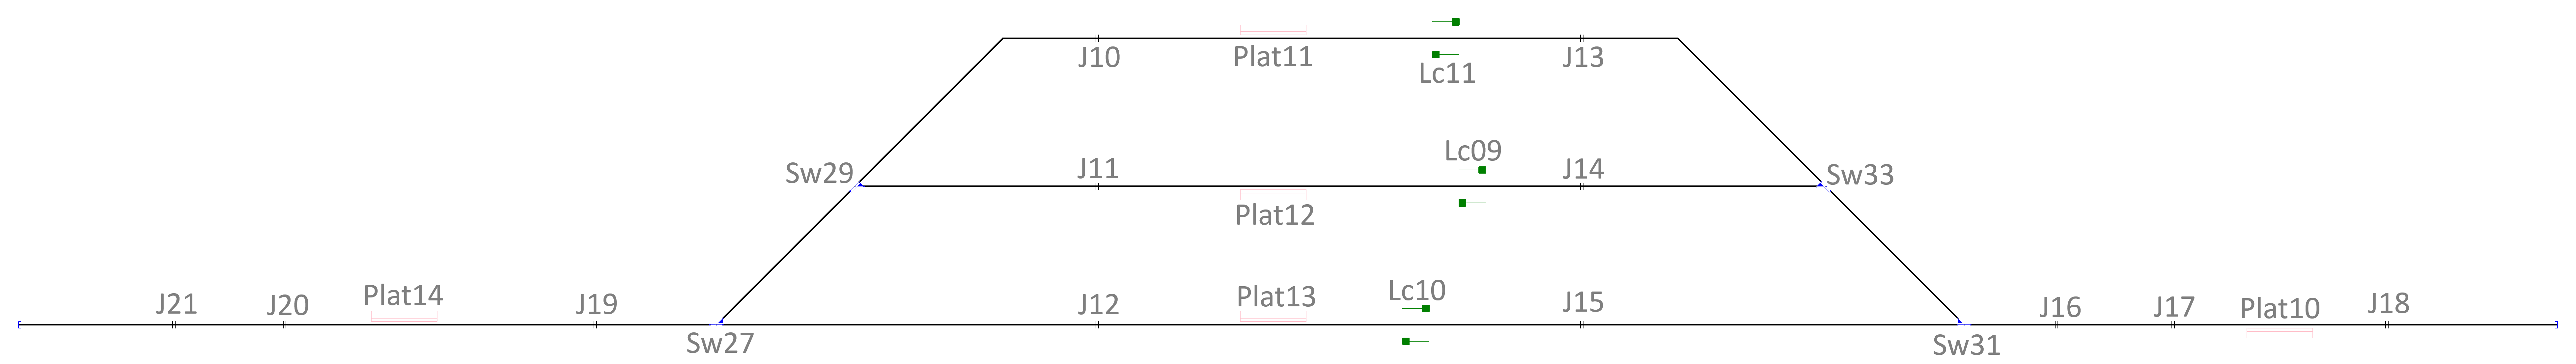
\includegraphics[width=1\textwidth]{resultados-obtenidos/ejemplo9/images/9_empty.png}
		\centering\caption{Topología ferroviaria del ejemplo 9 sin señalamiento.}
		\label{fig:EJ9_1}
	\end{figure}
	
	La topología presenta varias junturas entre los rieles, ya que el sistema original presentaba circuitos de vías y contadores de ejes, que fueron removidos para este ejercicio. No obstante, se mantienen las junturas para incrementar la dificultad del análisis.